\documentclass[12pt]{article}
\usepackage{amsthm}
\usepackage{amsmath}
\usepackage{array}
\usepackage{cancel}
\usepackage[thinc]{esdiff}
% \usepackage{gensymb}
\usepackage{geometry}
\usepackage{graphicx}
\usepackage{pgfplots}
\usepackage{siunitx}
\usepackage{wrapfig}
\usepackage{xcolor}

\title{Homework \#10, 4B}
\author{Donald Aingworth IV}
\date{March 26, 2025}

\pgfplotsset{width=8cm,compat=1.9}
\usepgfplotslibrary{external}
% \tikzexternalize

\renewcommand\thesubsection{\alph{subsection}}
\newcommand{\proj}{\text{proj}}
\newtheorem{theorem}{Theorem}

\begin{document}

\DeclareSIUnit{\mile}{mi}
\DeclareSIUnit{\gal}{gal}
\DeclareSIUnit{\foot}{ft}
\DeclareSIUnit{\hour}{h}
\DeclareSIUnit{\rad}{rad}
\DeclareSIUnit{\unit}{u}
\DeclareSIUnit{\dyne}{dyn}

\maketitle

\pagebreak
\section{Problem }
% \begin{wrapfigure}{r}{0.25\textwidth}
%     \vspace{-30pt}
%     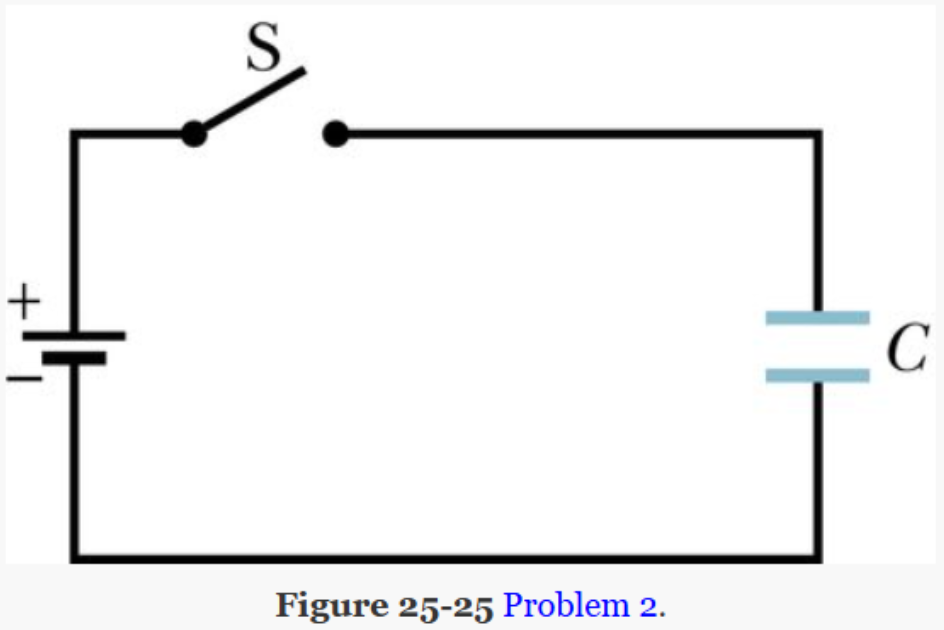
\includegraphics[width=0.25\textwidth]{picture_1.png} 
%     % \label{fig:wrapfig}
% \end{wrapfigure}


\subsection*{Solution}


\pagebreak

\end{document}